\opchapter{
    تحلیل پروژه
}\label{chap2}

\section{
    مقدمه
}\label{sec1:chap2}


\section{
    متدولوژی کنبان
}\label{sec2:chap2}
\lr{kanban}
\footnote{کَنبان.}
یک روش مدیریت چرخهٔ کار برای تعریف، مدیریت و بهبود سرویس‌های انتقال دانش کار است.
که هدف آن کمک برای متصور سازی، افزایش بهره‌وری و بهبود متداوم کار می‌باشد.

کنبان در زبان ژاپنی به معنی
\emph{تختهٔ بصری}
و یا
\emph{علامت}
است.
در ابتدا به عنوان یک سیستم برنامه‌ریزی به عنوان مدیریت ناب
\LTRfootnote{lean manufacturing \TNR\ /ˈli:n ˌmænjʊˈfæktʃərɪŋ/}
در سال
$1940$
توسط
\lr{Toyota}\footnote{
    تویوتا، یک ‌شرکت خودروسازی ژاپنی تأسیس شده در سال
    $1935$.
}
مطرح شد، که از سیستم همزمان
\lr{Toyota}
الهام گرفته شد، که بعد‌ها در سال
$2007$
به عنوان روش کنبان پدید آمد.
\cite{ohno1988toyota:book}
در متدولوژی کنبان از یک تخته کنبان استفاده می‌شود. 	در حالت ساده این تخته شامل $3$ ستون انجام دادن
(\lr{To-Do})،
در حال انجام
(\lr{In Progress})
و انجام شده
(\lr{Done})
است، که ممکن است شامل ستون‌های بانک اطلاعاتی
(\lr{Backlog})،
آماده انجام
(\lr{Ready})،
کد زنی
(\lr{Coding})،
آزمایش
(\lr{Testing})،
و تأ‌یید
(\lr{Approval})
نیز باشد.
\cite{kanbanize:online}

\emph{
کنبان برای یک
}\LTRfootnote{Kanban For 1.}،
یک روش الهام گرفته شده از کنبان مناسب برای توسعهٔ پروژه‌هایی با یک توسعه‌دهنده است.
\cite{prsonalkanban:online}
\begin{figure}[!h]
    \begin{center}
        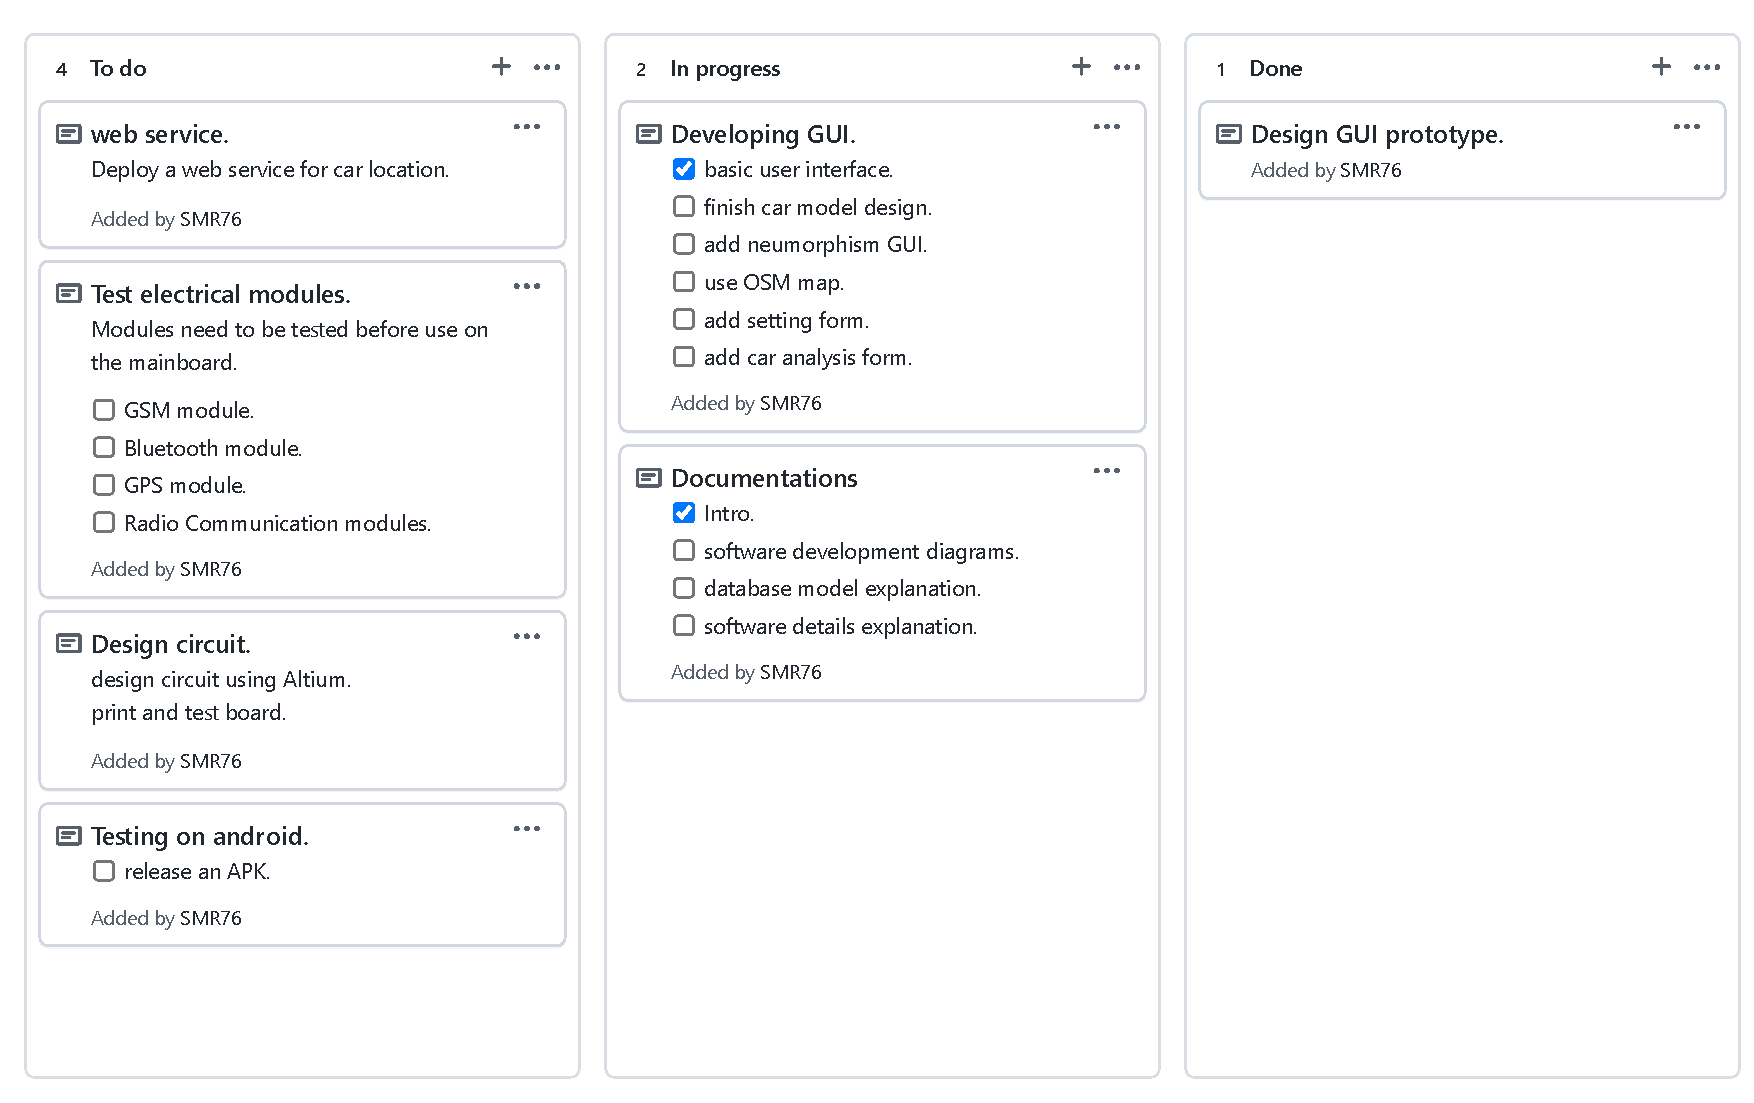
\includegraphics[width=0.8\textwidth]{images/kanban-board.pdf}
    \end{center}
    \caption{
        نمونهٔ تختهٔ کنبان در پروژهٔ جاری.
    }
    \label{fig3:sec1:chap2}
\end{figure}

\section{
    نمودار فعالیت
}\label{sec4:chap2}
نمودار فعالیت شامل عملکرد کاربر و طریقه انجام مراحل و گزینه‌های موجود پیش روی است.
این نمودار خلاصه‌ای از عملیات‌های موجود و قابل انجام توسط دستگاه را توضیح می‌دهد.

\begin{figure}[!h]
    \begin{center}
        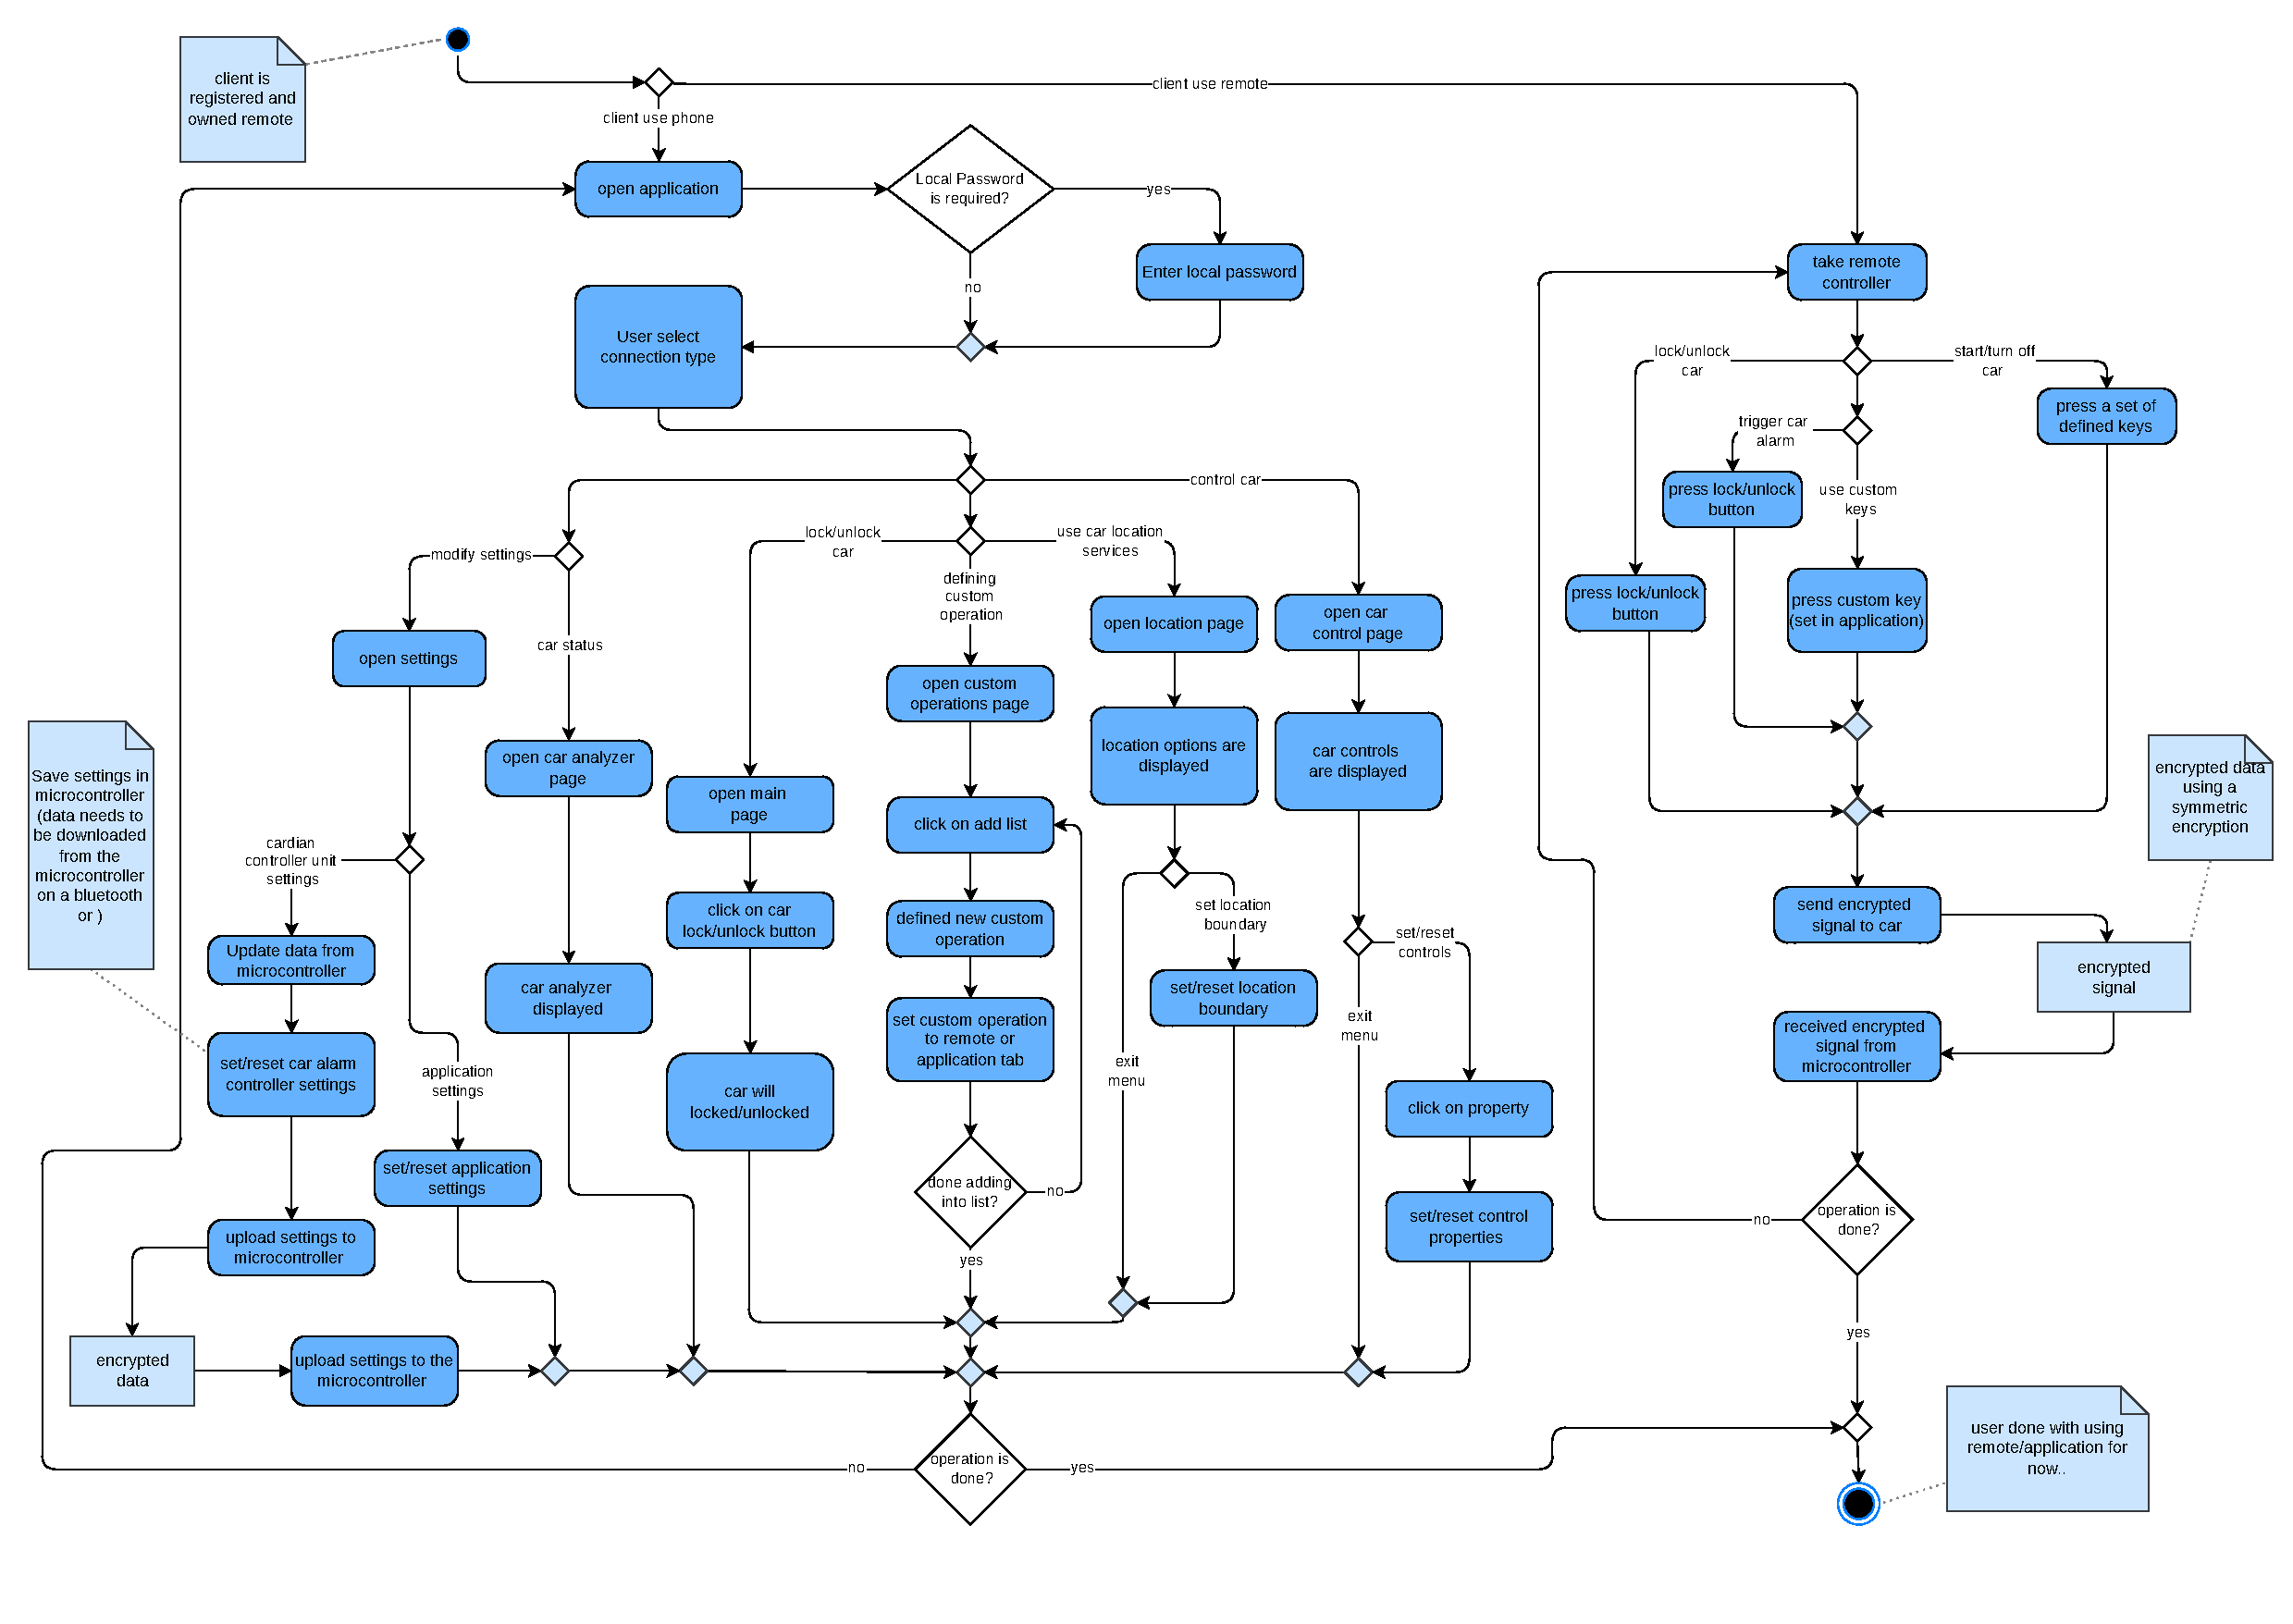
\includegraphics[width=0.8\textwidth]{../diagrams/activity-diagram.pdf}
        %../Extera/SD Diagrams/UML/activity-diagram.pdf
    \end{center}
    \caption{
    نمودار فعالیت.
    }
    \label{fig4:sec1:chap1}
\end{figure}

\pagebreak
\section{
    نمودار مدل و نشانه‌گذاری فرایند کسب‌وکار
}\label{sec5:chap2}

نمودار مدل و نشانه‌گذاری فرایند کسب‌وکار
(\lr{BPMN}\LTRfootnote{Business Process Model and Notation})
 یک نمودار گرافیکی است که برای نمایش و توصیف فرایندهای کسب و کار در یک سازمان استفاده می‌شود. این نمودارها با استفاده از یک مجموعه عناصر گرافیکی و قوانین نمونه سازی، نحوه جریان اطلاعات و وظایف در یک فرایند را نمایش می‌دهند.

نمودار
\lr{BPMN}
ترکیبی از اشکال گرافیکی و نمادهای استاندارد است که برای نشان دادن وظایف، دروازه‌ها، رویدادها، شروع و پایان فرایند، و نقش‌های مختلف در فرایند استفاده می‌شوند.

در زیر نمودار‌های از چند فرایند پروژه نمایش داده شده‌است:

\begin{figure}[!ht]
    \centering
    \footnotesize
    \begin{subfigure}[t]{0.47\linewidth}
        \centering
        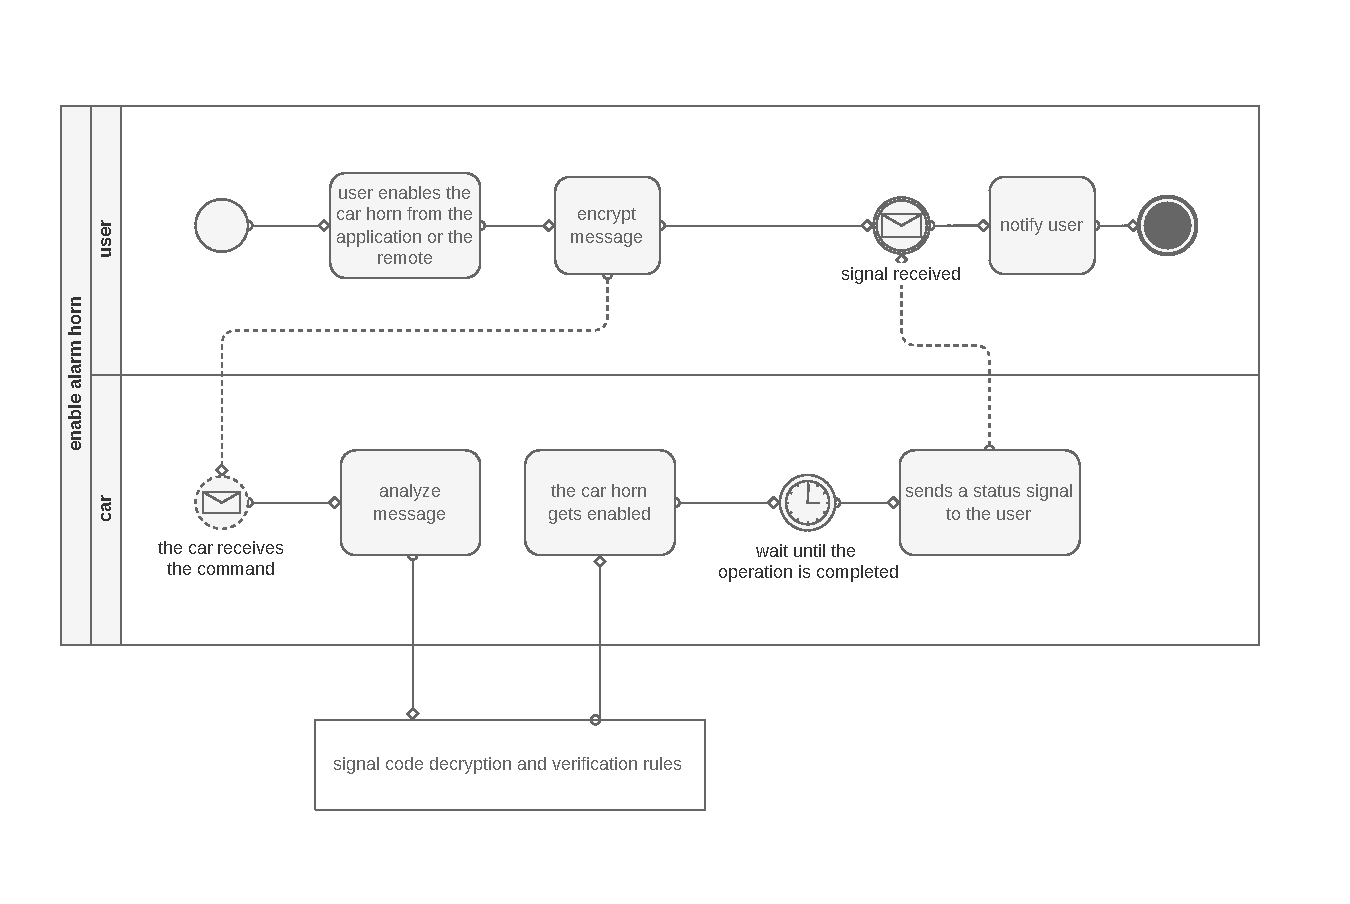
\includegraphics[width=\textwidth]{../diagrams/bpmn-diagram-1.pdf}
        \caption{
        فعال‌سازی آژیر خودرو
        }
        \label{subfig1:fig5:sec5:chap2}
    \end{subfigure}
    \begin{subfigure}[t]{0.47\linewidth}
        \centering
        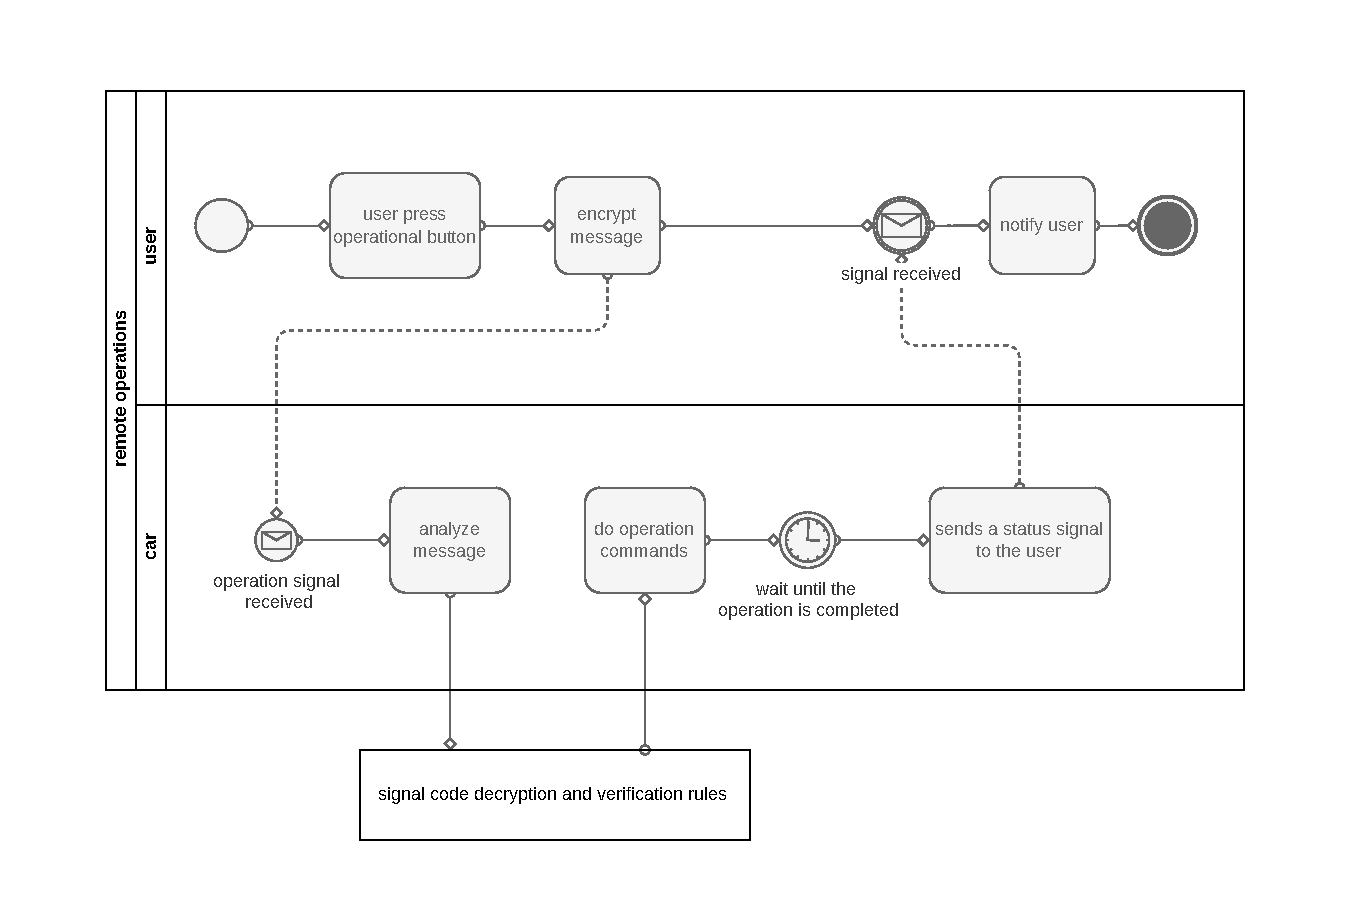
\includegraphics[width=\textwidth]{../diagrams/bpmn-diagram-2.pdf}
        \caption{
            مراحل کنترل از راه‌دور  خودرو
        }
        \label{subfig2:fig5:sec5:chap2}
    \end{subfigure}
    \hspace*{1cm}
    \normalsize
    \label{fig5:sec5:chap2}
    \caption{
        نمودار
        \lr{BPMN}
        بخش
        $2$
    }
\end{figure}

\begin{figure}[!ht]
    \centering
    \footnotesize
    \begin{subfigure}[t]{0.47\linewidth}
        \centering
        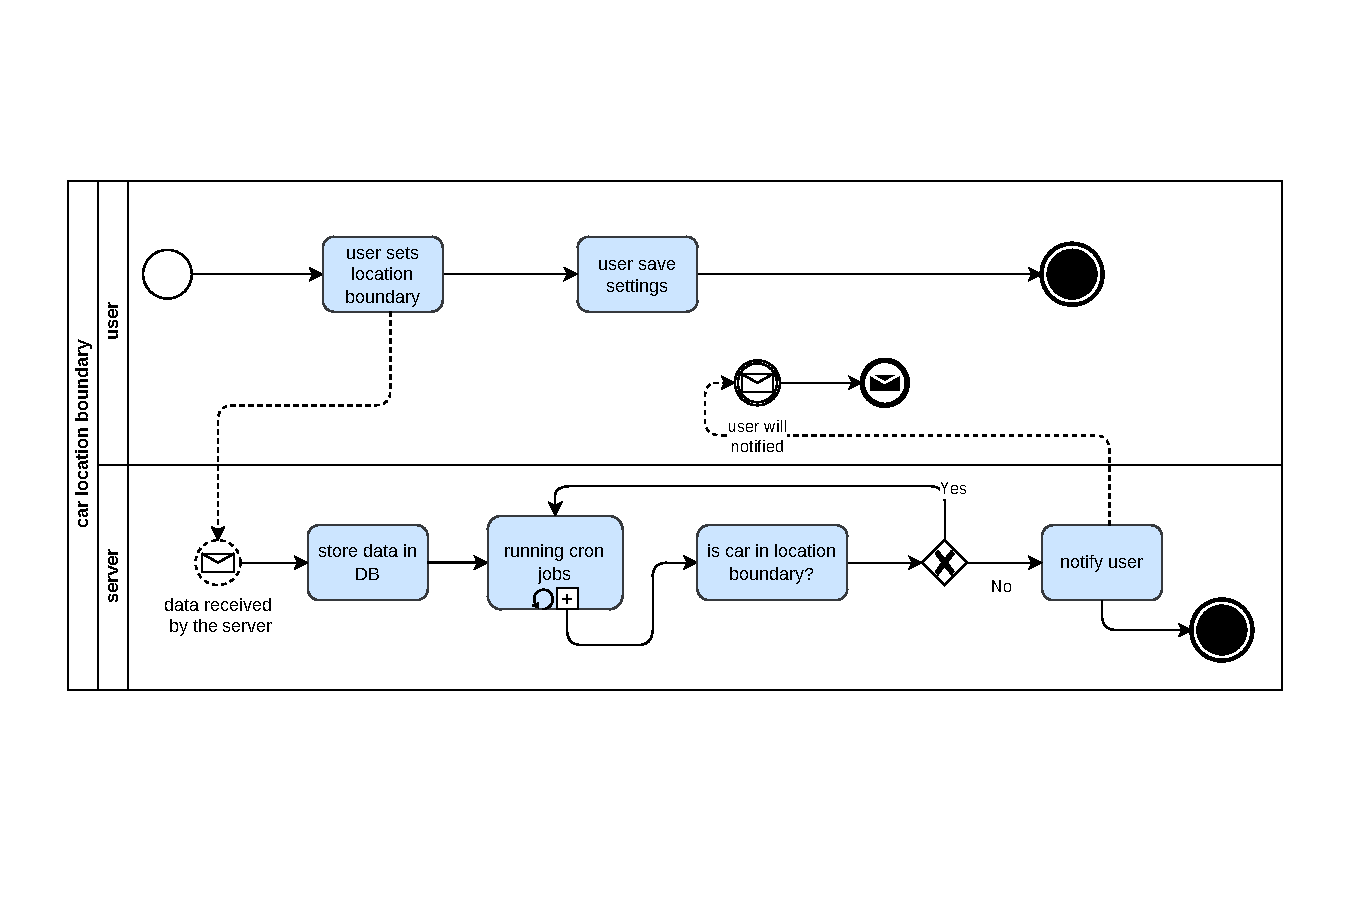
\includegraphics[width=\textwidth]{../diagrams/bpmn-diagram-3.pdf}
        \caption{
            قرار دادن محدودیت منطقه‌ای برای خودرو
        }
        \label{subfig1:fig6:sec5:chap2}
    \end{subfigure}
    \begin{subfigure}[t]{0.47\linewidth}
        \centering
        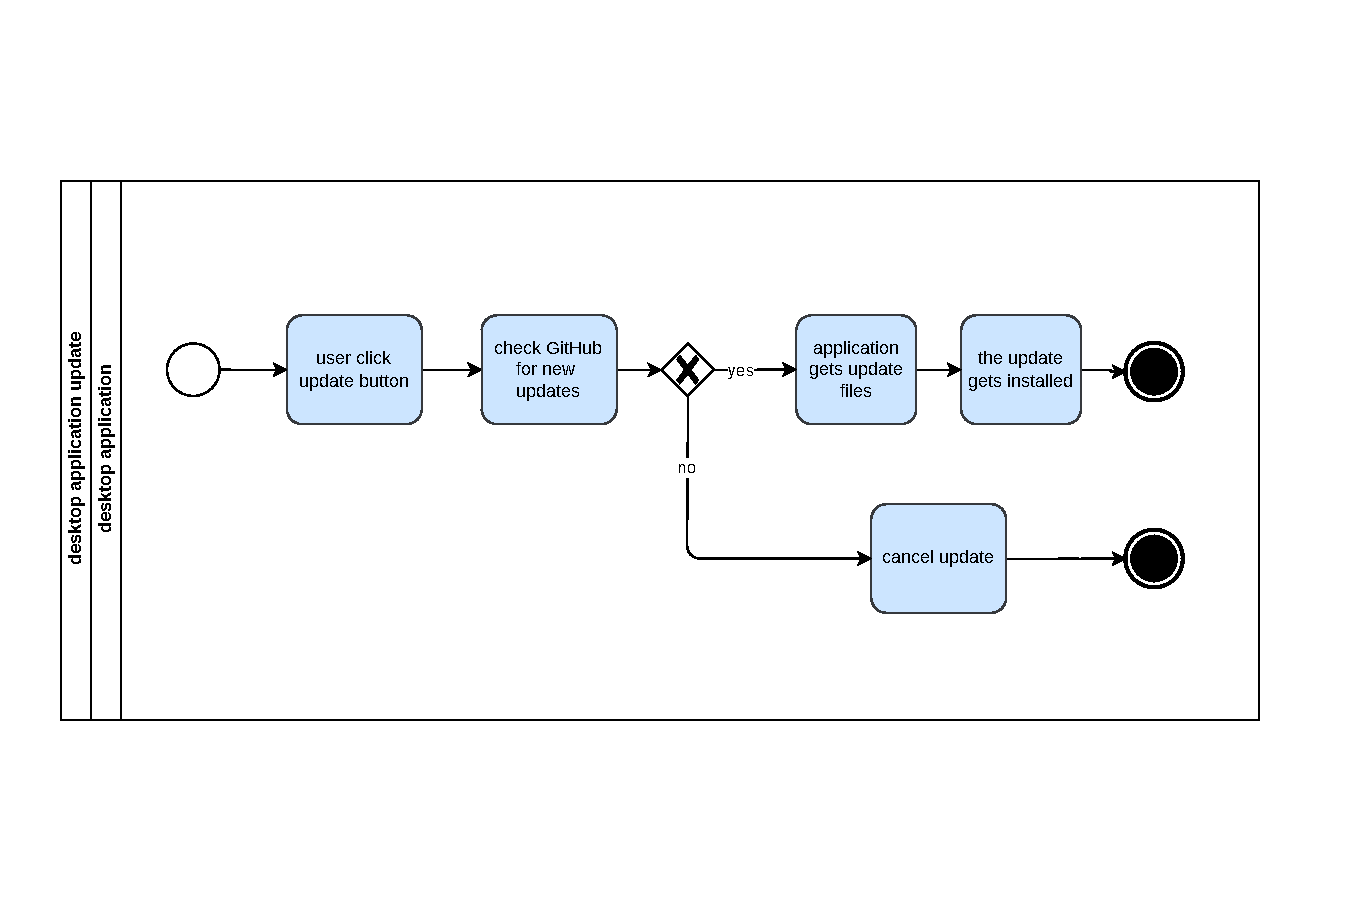
\includegraphics[width=\textwidth]{../diagrams/bpmn-diagram-4.pdf}
        \caption{
            به‌روزرسانی برنامهٔ
            \lr{desktop}
        }
        \label{subfig2:fig6:sec5:chap2}
    \end{subfigure}
    \hspace*{1cm}
    \normalsize
    \label{fig6:sec5:chap2}
    \caption{
        نمودار
        \lr{BPMN}
        بخش
        $1$
    }
\end{figure}